\documentclass[english]{SPFShortReport}
\usepackage{subfigure}
\usepackage{spfFigures}
\usepackage{longtable}
\usepackage{url}
\usepackage{gensymb}
\usepackage[yyyymmdd,hhmmss]{datetime}
\reportName{Python calculation for heat pump SI8TU}
\reportSubName{Parametric Heat Pump calculation} 
\reportDate{\today \hspace{0.1cm} at: \currenttime \hspace{0.1cm} h} 
\author{Dani Carbonell}
\address{dani.carbonell@solarenergy.ch}
\begin{document}
\begin{table}[!ht]
\begin{small}
\caption{Fitted coefficients for the heat pump.}
\begin{center}
\resizebox{12cm}{!} 
{
\begin{tabular}{l | c c } 
\hline
\hline
Coefficient &Description & \\ 
 & &$[kW]$\\ 
\hline
$PQ_{1}$ & \emph{$1^{st}$ condenser polynomial coefficient}  & 9.7100e+00    \\ 
$PQ_{2}$ & \emph{$2^{st}$ condenser polynomial coefficient}  & 7.1010e+01    \\ 
$PQ_{3}$ & \emph{$3^{st}$ condenser polynomial coefficient}  & -1.4100e+01    \\ 
$PQ_{4}$ & \emph{$4^{st}$ condenser polynomial coefficient}  & -7.1180e+01    \\ 
$PQ_{5}$ & \emph{$5^{st}$ condenser polynomial coefficient}  & 1.7675e+02    \\ 
$PQ_{6}$ & \emph{$6^{st}$ condenser polynomial coefficient}  & 1.4450e+01    \\ 
\hline
$PCOP_{1}$ & \emph{$1^{st}$ COP polynomial coefficient}  & 9.6700e+00    \\ 
$PCOP_{2}$ & \emph{$2^{st}$ COP polynomial coefficient}  & 7.4780e+01    \\ 
$PCOP_{3}$ & \emph{$3^{st}$ COP polynomial coefficient}  & -4.5480e+01    \\ 
$PCOP_{4}$ & \emph{$4^{st}$ COP polynomial coefficient}  & -2.2890e+02    \\ 
$PCOP_{5}$ & \emph{$5^{st}$ COP polynomial coefficient}  & 1.3432e+02    \\ 
$PCOP_{6}$ & \emph{$6^{st}$ COP polynomial coefficient}  & 6.9780e+01    \\ 
\hline
$\dot m_{cond}$ & 1400.00 $[kg/h]$\\ 
$\dot m_{evap}$ & 1930.00 $[kg/h]$\\ 
\hline
$COP_{nom}$ (B0W35)& 4.97 \\ 
$Q_{c,nom}$ (B0W35)& 7.89 kW\\ 
$COP_{nom}$ (B2W35)& 5.31 \\ 
$Q_{c,nom}$ (B2W35)& 8.32 kW\\ 
$COP_{nom}$ (B10W35)& 6.81 \\ 
$Q_{c,nom}$ (B10W35)& 10.22 kW\\ 
\hline
\hline
\end{tabular}
}
\label{CoefTable}
\end{center}
\end{small}
\end{table}
\begin{table}[!ht]
\begin{small}
\caption{Predicting results of the heat pump.}
\begin{center}
\resizebox{12cm}{!} 
{
\begin{tabular}{l | c c c c c c c c c c c } 
\hline
\hline
$T_{evap,in}$ &$T_{evap,out}$ &$T_{cond,in}$ &$T_{cond,out}$ &$COP$ &$Q_{cond}$ &$Q_{evap}$ &$W_{comp}$ &$\dot m_{cond}$ &$\dot m_{evap}$ &$\Delta T_{evap}$ &$\Delta T_{cond}$ \\ 
$^oC$ &$^oC$ &$^oC$ &$^oC$ &$[-]$ &$[kW]$ &$[kW]$ &$[kW]$ &kg/h &kg/h &K &K\\ 
\hline
-7.00 & -9.50 & 25.92 & 30.00 & 4.32 & 6.65 & 5.11 & 1.54 & 1400 & 1930 & 2.5 & 4.1\\ 
-7.00 & -9.26 & 34.82 & 38.75 & 3.62 & 6.40 & 4.63 & 1.77 & 1400 & 1930 & 2.3 & 3.9\\ 
-7.00 & -9.03 & 43.71 & 47.50 & 3.06 & 6.18 & 4.16 & 2.02 & 1400 & 1930 & 2.0 & 3.8\\ 
-7.00 & -8.82 & 52.58 & 56.25 & 2.65 & 5.98 & 3.72 & 2.26 & 1400 & 1930 & 1.8 & 3.7\\ 
-7.00 & -8.64 & 61.44 & 65.00 & 2.37 & 5.80 & 3.35 & 2.45 & 1400 & 1930 & 1.6 & 3.6\\ 
-4.00 & -6.80 & 25.56 & 30.00 & 4.80 & 7.23 & 5.73 & 1.51 & 1400 & 1930 & 2.8 & 4.4\\ 
-4.00 & -6.56 & 34.48 & 38.75 & 4.03 & 6.96 & 5.23 & 1.73 & 1400 & 1930 & 2.6 & 4.3\\ 
-4.00 & -6.31 & 43.38 & 47.50 & 3.39 & 6.71 & 4.73 & 1.98 & 1400 & 1930 & 2.3 & 4.1\\ 
-4.00 & -6.08 & 52.27 & 56.25 & 2.89 & 6.49 & 4.25 & 2.24 & 1400 & 1930 & 2.1 & 4.0\\ 
-4.00 & -5.86 & 61.14 & 65.00 & 2.54 & 6.30 & 3.81 & 2.48 & 1400 & 1930 & 1.9 & 3.9\\ 
-1.00 & -4.12 & 25.18 & 30.00 & 5.32 & 7.85 & 6.37 & 1.48 & 1400 & 1930 & 3.1 & 4.8\\ 
-1.00 & -3.86 & 34.11 & 38.75 & 4.46 & 7.55 & 5.86 & 1.69 & 1400 & 1930 & 2.9 & 4.6\\ 
-1.00 & -3.61 & 43.03 & 47.50 & 3.75 & 7.28 & 5.34 & 1.94 & 1400 & 1930 & 2.6 & 4.5\\ 
-1.00 & -3.36 & 51.93 & 56.25 & 3.17 & 7.04 & 4.82 & 2.22 & 1400 & 1930 & 2.4 & 4.3\\ 
-1.00 & -3.12 & 60.81 & 65.00 & 2.74 & 6.83 & 4.33 & 2.49 & 1400 & 1930 & 2.1 & 4.2\\ 
2.00 & -1.45 & 24.78 & 30.00 & 5.86 & 8.51 & 7.06 & 1.45 & 1400 & 1930 & 3.4 & 5.2\\ 
2.00 & -1.19 & 33.73 & 38.75 & 4.93 & 8.19 & 6.53 & 1.66 & 1400 & 1930 & 3.2 & 5.0\\ 
2.00 & -0.93 & 42.66 & 47.50 & 4.14 & 7.89 & 5.99 & 1.91 & 1400 & 1930 & 2.9 & 4.8\\ 
2.00 & -0.66 & 51.57 & 56.25 & 3.49 & 7.63 & 5.44 & 2.19 & 1400 & 1930 & 2.7 & 4.7\\ 
2.00 & -0.40 & 60.46 & 65.00 & 2.97 & 7.40 & 4.91 & 2.49 & 1400 & 1930 & 2.4 & 4.5\\ 
5.00 & 1.20 & 24.35 & 30.00 & 6.44 & 9.20 & 7.77 & 1.43 & 1400 & 1930 & 3.8 & 5.6\\ 
5.00 & 1.47 & 33.32 & 38.75 & 5.43 & 8.86 & 7.23 & 1.63 & 1400 & 1930 & 3.5 & 5.4\\ 
5.00 & 1.74 & 42.26 & 47.50 & 4.56 & 8.54 & 6.67 & 1.87 & 1400 & 1930 & 3.3 & 5.2\\ 
5.00 & 2.02 & 51.18 & 56.25 & 3.83 & 8.26 & 6.10 & 2.16 & 1400 & 1930 & 3.0 & 5.1\\ 
5.00 & 2.30 & 60.09 & 65.00 & 3.24 & 8.00 & 5.53 & 2.47 & 1400 & 1930 & 2.7 & 4.9\\ 
8.00 & 3.83 & 23.91 & 30.00 & 7.06 & 9.93 & 8.52 & 1.41 & 1400 & 1930 & 4.2 & 6.1\\ 
8.00 & 4.11 & 32.88 & 38.75 & 5.96 & 9.56 & 7.96 & 1.60 & 1400 & 1930 & 3.9 & 5.9\\ 
8.00 & 4.39 & 41.84 & 47.50 & 5.01 & 9.23 & 7.39 & 1.84 & 1400 & 1930 & 3.6 & 5.7\\ 
8.00 & 4.68 & 50.77 & 56.25 & 4.21 & 8.92 & 6.80 & 2.12 & 1400 & 1930 & 3.3 & 5.5\\ 
8.00 & 4.97 & 59.69 & 65.00 & 3.54 & 8.64 & 6.20 & 2.45 & 1400 & 1930 & 3.0 & 5.3\\ 
11.00 & 6.45 & 23.44 & 30.00 & 7.70 & 10.70 & 9.31 & 1.39 & 1400 & 1930 & 4.5 & 6.6\\ 
11.00 & 6.73 & 32.42 & 38.75 & 6.53 & 10.31 & 8.73 & 1.58 & 1400 & 1930 & 4.3 & 6.3\\ 
11.00 & 7.02 & 41.39 & 47.50 & 5.50 & 9.95 & 8.14 & 1.81 & 1400 & 1930 & 4.0 & 6.1\\ 
11.00 & 7.32 & 50.34 & 56.25 & 4.61 & 9.62 & 7.54 & 2.09 & 1400 & 1930 & 3.7 & 5.9\\ 
11.00 & 7.62 & 59.28 & 65.00 & 3.87 & 9.32 & 6.91 & 2.41 & 1400 & 1930 & 3.4 & 5.7\\ 
14.00 & 9.05 & 22.94 & 30.00 & 8.38 & 11.50 & 10.13 & 1.37 & 1400 & 1930 & 4.9 & 7.1\\ 
14.00 & 9.34 & 31.94 & 38.75 & 7.13 & 11.09 & 9.53 & 1.56 & 1400 & 1930 & 4.7 & 6.8\\ 
14.00 & 9.63 & 40.93 & 47.50 & 6.02 & 10.71 & 8.93 & 1.78 & 1400 & 1930 & 4.4 & 6.6\\ 
14.00 & 9.94 & 49.89 & 56.25 & 5.05 & 10.36 & 8.31 & 2.05 & 1400 & 1930 & 4.1 & 6.4\\ 
14.00 & 10.25 & 58.84 & 65.00 & 4.23 & 10.04 & 7.67 & 2.38 & 1400 & 1930 & 3.7 & 6.2\\ 
17.00 & 11.63 & 22.43 & 30.00 & 9.09 & 12.34 & 10.98 & 1.36 & 1400 & 1930 & 5.4 & 7.6\\ 
17.00 & 11.93 & 31.44 & 38.75 & 7.76 & 11.91 & 10.37 & 1.54 & 1400 & 1930 & 5.1 & 7.3\\ 
17.00 & 12.23 & 40.44 & 47.50 & 6.57 & 11.51 & 9.76 & 1.75 & 1400 & 1930 & 4.8 & 7.1\\ 
17.00 & 12.54 & 49.42 & 56.25 & 5.53 & 11.14 & 9.12 & 2.02 & 1400 & 1930 & 4.5 & 6.8\\ 
17.00 & 12.87 & 58.38 & 65.00 & 4.62 & 10.79 & 8.46 & 2.34 & 1400 & 1930 & 4.1 & 6.6\\ 
20.00 & 14.20 & 21.89 & 30.00 & 9.83 & 13.22 & 11.87 & 1.34 & 1400 & 1930 & 5.8 & 8.1\\ 
20.00 & 14.50 & 30.92 & 38.75 & 8.42 & 12.76 & 11.25 & 1.52 & 1400 & 1930 & 5.5 & 7.8\\ 
20.00 & 14.81 & 39.93 & 47.50 & 7.16 & 12.34 & 10.62 & 1.72 & 1400 & 1930 & 5.2 & 7.6\\ 
20.00 & 15.13 & 48.92 & 56.25 & 6.03 & 11.95 & 9.97 & 1.98 & 1400 & 1930 & 4.9 & 7.3\\ 
20.00 & 15.46 & 57.89 & 65.00 & 5.05 & 11.58 & 9.29 & 2.29 & 1400 & 1930 & 4.5 & 7.1\\ 
\hline
\hline
\end{tabular}
}
\label{ResultsTable}
\end{center}
\end{small}
\end{table}
\begin{figure}[!ht]
\begin{center}
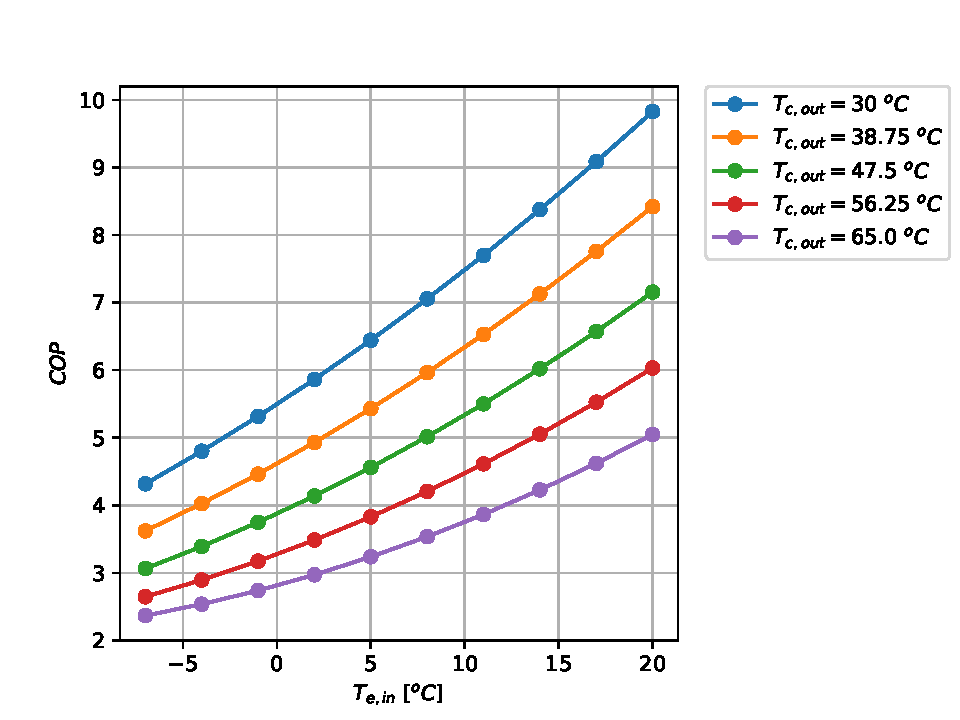
\includegraphics[width=1\textwidth]{C:/Daten/spfPackages/GIT/spfTrnsysFiles/HeatPump/BrineToWater/LEXETA/SI8TU/SI8TU-Cop.pdf}
\caption{COP Results for the heat pump at the selected points}
\label{COPFig}
\end{center}
\end{figure}
\begin{figure}[!ht]
\begin{center}
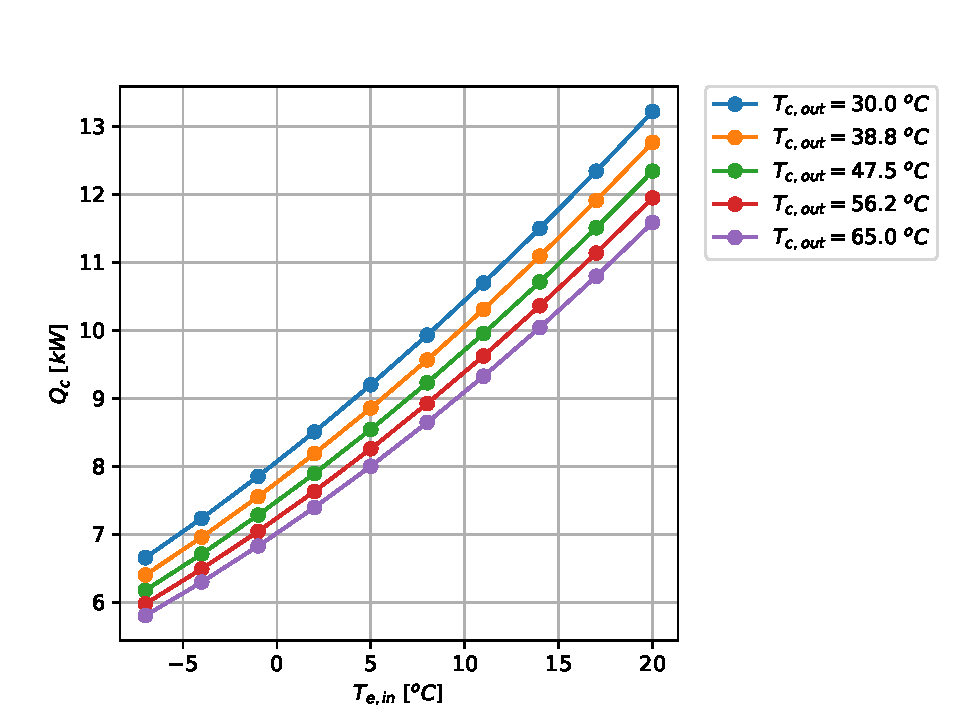
\includegraphics[width=1\textwidth]{C:/Daten/spfPackages/GIT/spfTrnsysFiles/HeatPump/BrineToWater/LEXETA/SI8TU/SI8TU-Qc.pdf}
\caption{$Q_c$ Results for the heat pump at the selected points}
\label{QcFig}
\end{center}
\end{figure}
\end{document}
